%!TEX root = /Users/markelikalderon/Documents/Git/formwithoutmatter/aristotle.tex
\chapter{Perception at a Distance} % (fold)
\label{cha:perception_at_a_distance}

In its original form, Empedoclean puzzlement about the sensory presentation of remote objects consists in the apparent tension between two claims:
\begin{enumerate}[(1)]
    \item The objects of color perception are qualities of external particulars located at a distance from the perceiver.
    \item \emph{The Empedoclean principle}: To be perceptible is to be palpable to sense---in order for something to be the object of perception it must be in contact with the relevant sense organ.
\end{enumerate}
Short of embracing the theory of effluences, how might one respond to Empedoclean puzzlement as it arises in its original form? Either (1) or (2) may be rejected, or an alternative reconciliation may be proposed, one not involving the assimilation of material effluences.

In case it is unobvious that anyone would reject (1), Parmenides may count among its deniers. Specifically, Parmenides (\textsc{dk} 28\textsc{b}8.41) claims that it merely appears that things alter their color. The Way of Mortal Opinion, in maintaining otherwise, conflates appearance with reality. Strictly speaking, this claim is consistent with remote external particulars having unchanging colors. However, if we bear in mind the broader philosophical context, at least as standardly interpreted, it is plausible that Parmenides meant to deny not just that things alter their color as they appear to do, but that things are colored at all. Colors are qualities that appear in sensory experience and are in this sense part of the sensible world. The sensible world is associated with becoming as opposed to being. Perhaps, the underlying thought is that it is characteristic of sensory experience that it presents us with a flux of sensible qualities. Sensible qualities, qualities that appear in sensory experience, are subject to change. Since change is impossible, things merely appear to have sensible qualities. The attributes of the one being of The Way of Truth are intelligible as opposed to sensible. There are thus no qualities of external particulars that are the objects of color perception. On Palmer's \citeyearpar{Palmer:2009qf} alternative modal interpretation, external objects retain their sensible qualities, it is just that sensible qualities would not inhere in things with a distinctive mode of being characteristic of things which exist necessarily. Whereas a necessary being is ungenerated, imperishable, and unchanging, the objects that we perceive are contingent beings and thus are generated, perishable, and subject to change. Thus perception at best affords us an understanding that ``wanders'', that varies with its object's every change. Even if Palmer is right about Parmenides, the denial of (1) along the lines sketched above would plausibly be found in a sophistical treatment of this Eleatic topic.

Despite his shift to a pluralist metaphysics, Democritus retains an Eleatic color irrealism (be it of genuine Parminidean provenance or a sophistical take on Eleatic material). Concerning Democritus, Sextus Empiricus reports:
\begin{quote}
	And Democritus in some places abolishes the things that appear to the senses and asserts that none of them appears in truth but only in opinion, the true fact in things existent being the existence of atoms and void; for ``By convention,'' he says, ``is sweet, by convention bitter, by convention hot, by convention cold, by convention color; but by verity atoms and void.'' (This means: Sensible objects are conventionally assumed and opined to exist, but they do not truly exist, but only the atoms and the void.) (Sextus Empiricus, \emph{Against the Logicians}, \emph{adv. math.}, \textsc{vii}; \citealt[135--136]{Bury:1997uq}) 
\end{quote}
According to the interpretation offered by Sextus Empriricus, linguistic conventions may license, in certain circumstances, our predicating ``white'' of the sun given the character of the sensory experience it elicits, but there is nothing corresponding to this predication over and above this sensory reaction to atomic stimuli. There are thus no qualities of external particulars that are the objects of color perception. 

Parmenides and Democritus deny (1) by denying the existence of the colors. A more modern denial of (1) retains the existence of the colors but denies that they are qualities of external particulars. Thus while \citet{Berkeley:1734fk} maintains that colors are the objects of sight, he denies that they are qualities inherent in external bodies. \citet{Berkeley:1744rm} himself cites ancient precedent for this doctrine. In particular he advances an interpretation of the Secret Doctrine of the \emph{Theaetetus} that would support this denial and so credits Protagoras as an adherent. But as \citet{Burnyeat:1982mz} argues, the claim to ancient precedent is spurious, and the denial is distinctly modern. Berkeley maintains that the object of perception depends upon the perceiving subject. Indeed, the being of color wholly consists in its being seen. But, according to the Secret Doctrine of Protagoras, the perception itself depends upon its objects. Protagoras is represented as positing a mutual dependence between perception and object perceived. Sense and sensibilia are correlatives in a way that Berkeley never conceives of them.

In addition, instead of rejecting either (1) or (2), one may propose an alternative reconciliation, one not involving the assimilation of effluences. Instead of the perceiver assimilating material effluences, perhaps perception can be understood in terms of the perceiver emitting them. Thus Aristotle attributes to Empedocles and Plato in the \emph{Timaeus} accounts of perception that involve the eye's emission of fiery effluences. And within the distinct tradition of geometrical optics, thinkers such as Euclid, Hero, Galen, and Ptolemy, used lines determined by visual rays emitted from the eye as the basis of geometrical reasoning in offering explanations of reflection, the variation in apparent size with distance, and the rudiments of perspective. Moreover, such reasoning possibly had effective military application, if stories about Archimedes' burning mirror are to be believed. Effluences or visual rays emitted by the eye reconcile the ingestion model with sensible objects being remote by themselves being a kind of extended ethereal touch. Emission would be a means of reaching out so as to grasp the sensible object. On this alternative, sight is conceived the way Diderot's blind man conceives of it: ``This blind man's only knowledge of objects is by touch. \ldots\ Sight, he therefore concludes, is a kind of touch which extends to distant objects'' (Diderot, ``Letter on the Blind for the Use of Those Who See''; \citealt[72]{Jourdain:1916aa}). Aristotle will rightly complain that this extended ethereal touch is not well explained and so could not be understood as the mode of perceptual apprehension that its advocates present it as being.

Aristotle clearly accepts (1)---that the objects of color perception are qualities of external particulars located at a distance from the perceiver. Importantly, this is the result, in part, of some fundamental commitments that Aristotle undertakes with respect to the nature of our perceptual capacities and their objects. Moreover, when combined with the Empedoclean principle, to be perceptible is to be palpable to sense, it generates precisely the puzzlement that the theory of effluences is designed to resolve. However, Aristotle rejects Empedocles' theory of effluences. And with no viable alternative reconciliation to hand, Aristotle is committed to rejecting (2). 

The nature of Aristotle's case is our present topic. First, we will discuss the fundamental commitments about our perceptual capacities and their objects that underly Aristotle's acceptance of (1)---that the objects of color perception are qualities of external particulars located at a distance from the perceiver. Second, we will discuss Aristotle's argument against (2)---the Empedoclean principle that to be perceptible is to be palpable to sense. As we shall see, according to Aristotle, not only is the Empedoclean principle an overgeneralization from a paradigm case, but a misconception of it as well. Third, Empedoclean puzzlement, in its most general form, survives the rejection of the principle that to be perceptible is to be palpable to sense. There thus remain unanswered questions in rejecting (2). Moreover, these questions partly set the agenda in Aristotle's discussion of perception (the present essay, as a whole, constitutes an argument for this latter claim). 

\section{The Sensible Qualities of Remote External Particulars} % (fold)
\label{sec:sensible_qualities_of_remote_external_particulars}

Color perception involves the visual presentation of qualities of remote external particulars. The particulars are external in that they exist and have their natures and powers independently of the perceiver. The relevant sense of independence may guarantee that the perceiver and the particular are spatially non-coincident (since two bodies cannot occupy the same space at the same time, \emph{De Anima} \textsc{ii} 7 418\( ^{b} \)19), but it does not guarantee that they are non-contiguous. Spatially non-coincident bodies may yet be in contact with one another. Thus talk of remote external particulars is not redundant. Their remoteness consists in the non-contiguity of the perceiver and external particular.

In this section we shall discuss the general reasons that underly Aristotle's commitment to three claims:
\begin{enumerate}[(1)]
    \item The objects of perception are external;
    \item The objects of perception are particulars and their qualities;
    \item The objects of perception are remote.
\end{enumerate}
Taken together they explain Aristotle's commitment to the objects of color perception being qualities of external particulars located at a distance from the perceiver. It is the conjunction of this commitment and the Empedoclean principle that generates the puzzlement that Empedocles' theory of effluences was designed to resolve.

\subsection{External} % (fold)
\label{sub:external}

Sensible qualities inhere in external particulars. They are external in that they exist and have the natures and powers they do independently of being perceived. The relevant sense of independence is usefully highlighted by contrasting Aristotle's position with Protagoras'.

Protagoras notoriously claims that man is the measure of all things. According to Plato's \emph{Theaetetus} and Aristotle's \emph{Metaphysica} \( \Gamma \), Protagoras' measure doctrine is supported by an account of perception where neither the perceptual experience nor the object of perception takes precedence over one another. Perception and the object of perception, so understood, are correlatives. Moreover, this account of the relation between perception and its object is meant to have the startling consequence that nothing we perceive exists prior to our perception. Perhaps surprisingly, Aristotle accepts that perception and its object are correlatives. Nevertheless, on his own account of relatives, the startling Protagorean consequence is avoided. Indeed, consistent with perception and the perceptible being correlatives, Aristotle maintains that the perceptible is prior to perception, the sensible is prior to sensation.

In \emph{Categoriae} \textsc{vii}, Aristotle defines \emph{relatives} as follows:
\begin{quote}
    We call \emph{relatives} all such things as are said to be just what they are, \emph{of} or \emph{than} things, or in some other way \emph{in relation to} something else. (Aristotle, \emph{Categoriae} \textsc{vii} 6\( ^{a} \)37; Ackrill in \citealt[11]{Barnes:1984uq})
\end{quote}
So understood, relatives are not relations, but relational categories---categories that only apply because some relation obtains. They are ways for things to be that wholly depend upon a thing's relations. Being related to something else is what it is to be relative to that thing. Thus to be a perception is for the perceiver to be perceptually related to an object of perception. And for something to be an object of perception is for it to be what the perceiver is perceptually related to. Thus a perception is in this sense relative to its object and the object of perception is relative to the perception whose object it is. Aristotle further holds that ``All relatives are spoken of in relation to correlatives that reciprocate'' (\emph{Categoriae} \textsc{vii} 6\( ^{b} \)28; Ackrill in \citealt[11]{Barnes:1984uq}) provided that they are properly given (\emph{Categoriae} \textsc{vii} 7\( ^{a} \)22--23). Thus the larger is larger than the smaller and the smaller is smaller than the larger. Aristotle explains the constraint that correlatives that reciprocate be properly given as follows:
\begin{quote}
    For example, if a wing is given as \emph{of a bird}, \emph{bird of a wing} does not reciprocate; for it has not been given properly in the first place as wing of a bird. For it is not as being a bird that a wing is said to be of it, but as being a winged, since many things that are not birds have wings. Thus if it given properly there is reciprocation; for example, a wing is wing of a winged and a winged is winged with a wing. (Aristotle, \emph{Categoriae} \textsc{vii} 6\( ^{b} \)38--7\( ^{a} \)5; Ackrill in \citealt[12]{Barnes:1984uq})
\end{quote}
A bird is a winged, but the relative that reciprocates is only properly given in terms of the relevant underlying relation. To be a wing is to be related in a certain way to something as its wings, that is to say, to a winged---something considered only in so far as it bears the winged relation to a wing. A bird does not reciprocate a wing since there are things with wings that are not birds. Being a bird does not wholly consists in having wings as parts and so is not a correlative.

According to Aristotle, sense and sensibilia, perception and the perceptible, are correlatives, as are knowledge and the knowable. Perceptual and epistemic correlatives differ from other correlatives in two important ways, however. First, Aristotle observes that: ``knowledge is called knowledge \emph{of} what is knowable, and what is knowable knowable \emph{by} knowledge; perception perception \emph{of} the perceptible, and the perceptible perceptible \emph{by} perception'' (\emph{Categoriae} \textsc{vii} 6\( ^{b} \)28--36; Ackrill in \citealt[11--12]{Barnes:1984uq}). Knowledge and perception are alike in that each takes an object, and they differ in this way from other correlatives, such as the larger and the smaller, the wing and the winged. 

Second, Aristotle argues that the perceptible must be prior to perception:
\begin{quote}
    The perceptible seems to be prior to perception. For the destruction of the perceptible carries perception to destruction, but perception does not carry the perceptible to destruction. For perceptions are to do with body and in body, and if the perceptible is destroyed, body too is destroyed (since body is itself a perceptible), and if there is not body, perception too is destroyed; hence the perceptible carries perception to destruction. But perception does not carry the perceptible. For if animal is destroyed perception is destroyed, but there will be something perceptible, such as body, hot, sweet bitter, and all the other perceptibles. Moreover, perception comes into existence at the same time as what is capable of perceiving---an animal and perception come into existence at the same time---but the perceptible exists before perception exists; fire and water and so on, of which an animal is itself made up, exist even before there exists an animal at all, or perception. Hence the perceptible would seem to be prior to perception. (Aristotle, \emph{Categoriae} \textsc{vii} 7\( ^{b} \)35--8\( ^{a} \)13; Ackrill in \citealt[13--14]{Barnes:1984uq})
\end{quote}
Perception and the perceptible, sense and sensibilia, may be correlatives, but that is consistent with the following asymmetry---the perceptible can exist prior to perception and so does not depend upon perception the way perception depends upon its object. Aristotle gives arguments for two claims: (1) that perception existentially depends upon the perceptible, and (2) that the perceptible does not existentially depend upon perception. Taken together (1) and (2) entail that the perceptible is existentially prior to perception.

The argument for (1) takes an interesting and perhaps unexpected form. One might have expected Aristotle to argue that since perception essentially takes an object there must be something that the perception, or perhaps the perceiver, is perceptually related to. Thus if the perceptible, understood as potential \emph{relata} of the perceptual relation, does not exist, neither does any perception of them. But that is not, in fact, how Aristotle argues. Aristotle emphasizes, instead, that perceptions are the exercises of perceptual capacities possessed by certain natural bodies, namely, animals. These bodies---the bodies that possess perceptual capacities, capacities whose proper exercise consists in the presentation of their primary objects, color for sight, sound for hearing---are themselves perceptible. So if nothing perceptible exists, nothing in fact has the capacity to perceive. And if nothing has the capacity to perceive, there are no perceptions.

The argument for (2) is more straightforward but retains the focus on certain natural bodies, animals, understood as the possessor's of perceptual capacities. Suppose there are no animals. Then nothing possesses the capacity to perceive. And if nothing has the capacity to perceive, there are no perceptions. Nevertheless, consistent with the absence of perceivers, the perceptible would persist. An Extinction Level Event may destroy all animal life, and, hence, all perceivers, on Earth, but things would remain white, or hot, or bitter. Things would continue to be the way they are in observable respects even in the absence of perceivers.

Towards the end of the passage from the \emph{Categoriae}, Aristotle adds a third claim: (3) Not only is the perceptible existentially prior to perception, but the perceptible is temporally prior as well. And again, there is a focus on certain natural bodies that possess perceptual capacities. Animals, natural bodies with perceptual capacities, have an elemental composition. Animals are composed of the so-called elements, such as fire and water. Fire and water, like the animals that are composed of them, are perceptible. Before the animal is composed of its elements, and so comes to possess perceptual capacities and so perceive, the elements out of which the animal is composed would exist and be the potential objects of perception. And so Aristotle concludes that the perceptible is not only existentially prior to perception but temporally prior as well.

The arguments in the \emph{Categoriae} for (1)--(3) all emphasize that perception, though it may involve the presentation of the perceptible in sense experience, is nevertheless to be understood as the exercise of a capacity possessed by certain animate natural bodies, animals if not plants. The corresponding arguments in the \emph{Metaphysica} will themselves emphasize that perception is the exercise of a capacity possessed by animals. However, in the \emph{Metaphysica}, there is a crucial shift of focus. While in the \emph{Categoriae}, Aristotle emphasizes the way in which the natural bodies that possess perceptual capacities, and the elements that compose these bodies, are themselves perceptible, in the \emph{Metaphysica}, however, Aristotle emphasizes instead the kind of capacity involved in perceiving the environment. 
Specifically, sensory capacities are a mode of sensitivity to sensible aspects of the natural environment. As such they are reactive capacities, they only ever act by reacting to the presence, in their environment, of the sensible object. So there is a shift of focus from certain natural bodies possessing perceptual capacities to the objects that trigger the exercise of these capacities.

% A perception is an encounter in sense experience with at least the primary object of the sensory modality. 

That the objects of perception are independent of perceivers perceiving them is brought out clearly in one of a battery of arguments that Aristotle brings to bear against Protagoras in \emph{Metaphysica} \( \Gamma \):
\begin{quote}
	And, in general, if only the sensible exists, there would be nothing if animate things were not; for there would be no faculty of sense. Now the view that neither the sensible qualities nor the sensations would exist is doubtless true (for they are affections of the perceiver), but that the substrata which cause the sensation should not exist even apart from sensations is impossible. For sensation is surely not the sensation of itself, but there is something beyond the sensation, which must be prior to the sensation; for that which moves is prior in nature to that which is moved, and if they are correlative terms, this is no less the case. (Aristotle, \emph{Metaphysica} \( \Gamma \) 5 1010\( ^{b} \)30--1011\( ^{a} \)2; Ross in \citealt[55--56]{Barnes:1984kx})
\end{quote}
Aristotle's target is the claim that only the sensible exists, a doctrine that Aristotle ascribes to a number of early thinkers but sees exemplified by Protagoras' measure doctrine. 

In the initial portion of the passage, the claim that nature is restricted to its sensible aspects is subject to a \emph{reductio ad absurdum}. If only what can be perceived exists, then if no animals existed, nothing would be perceived, since animals are the only natural bodies that possess the capacity to perceive. From which it is meant to follow that nothing could exist. Whether the conclusion follows depends on the sense of the thesis assumed for the sake of \emph{reductio}. How are we to understand the claim that only the sensible exists? The conclusion of the \emph{reductio} would follow from the principle that:
\begin{quote}
	If something exists, then it is perceived
\end{quote}
since a world without animals is a world without perception. Perhaps the claim that only the sensible exists can be understood in terms of the weaker principle:
\begin{quote}
	If something exists, then it is possible that it is perceived 
\end{quote}
Would the conclusion of the \emph{reductio} follow from the weaker principle? Whether it does depends on the sense of possibility involved. In a world without perceivers, given how things are in such a world, it is not possible for anything to be perceived. In order for something to be perceived, there must be perceivers, but there are none. The weaker principle, understood in terms of this sense of possibility, would suffice for the conclusion of the \emph{reductio}. Nevertheless, in a world without perceivers, there is another reasonable sense in which it is possible for something to be perceived. Even if no perceivers existed for the rest of eternity, the particulars in the natural environment could be of such a nature, or possess such a power, that had there been perceivers, they could have been perceived. This latter thought is no aid to the Protagorean, however. Aristotle thinks that the envisioned possibility is only intelligible against the background of a realist metaphysics. Aristotle concedes to Protagoras that neither sensible qualities nor perceptions would exist if no perceivers exist. There certainly would be no sensible qualities as Protagoras conceives of them, at least if he is a perceptual relativist. But even if no perceivers exist, there would remain a ``substrata'' which retains the power to cause perceptions in animals with suitable sensory capacities. 

Aristotle provides metaphysical and phenomenological grounds for the existence of such substrata. The metaphysical grounds turn on the kind of capacity perceptual capacities are, reactive capacities, at least if perception is a mode of sensitivity to the sensible aspects of the natural environment. If perception is a mode of sensitivity, as it must be if it is to be perception at all, the objects of perception must exist independently of perception and be the potential cause of perception. A reactive capacity only acts by reacting. The possessor of the reactive capacity must be acted upon before their reactive capacity can be exercised. And what acts upon the possessor of the reactive capacity must exist prior to the reaction it elicits. Not only does Aristotle provide metaphysical grounds for the existence of substrata, arguably at least, he provides phenomenological grounds as well: 
\begin{quote}
	For sensation is surely not the sensation of itself, but there is something beyond the sensation, which must be prior to the sensation. (\emph{Metaphysica} \( \Gamma \) 6 1011\( ^{a} \)1; Ross in \citealt[56]{Barnes:1984kx})
\end{quote}
Given the phenomenology of our perceptual experience, perception seems to present us with objects that exists independently of perception. Our sense experience seems to present us something beyond the sensation. Moreover, it does so by presenting itself as a mode of sensitivity to how things are, in sensible respects, independently of the perceiver.

It is unclear what Aristotle means by ``substrata''. Does he mean persisting particular bodies like artifacts and natural objects? Or does he mean something broader in this context, broad enough to include not only external particulars but their qualities as well? Just because particulars must be independent causes of perception, it does not follow that they possess their sensible qualities independently of perception, or that their qualities can themselves be the cause of perception. If, on the other hand, in the argument against Protagoras, ``substrata'' is meant to include not only external particulars but their sensible qualities, then external particulars possess their sensible qualities independently of being perceived. 

Can sensible qualities, or at least their instances, cause perception? If so, they are among the substrata that exist independently of perception. If colors exist independently of being perceived, this is strong prima facie evidence that Aristotle is committed to the kind of color realism that the early moderns, such as Descartes, Boyle, and Locke, rejected. There are other passages, however, that can seem to conflict with this interpretation. Whether Aristotle is, in fact, a color realist, and in what sense, will be determined later.

The discussion in \emph{Metaphysica} \( \Delta \) suggests this broader interpretation.
\begin{quote}
	Similarly, sight is the sight of something, not `of that of which it is the sight' (though of course it is true to say this); in fact it is relative to color or to something else of the sort. But according to the other way of speaking the same thing would be said twice---`the sight is of that of which it is'. (Aristotle, \emph{Metaphysica} \( \Delta \) 15 1021\( ^{a} \)34--1021\( ^{b} \)3; Ross in \citealt[76]{Barnes:1984kx})
\end{quote}
Perception is relative to its object, in the case of sight, it is relative to the perceived color. In order for sight to be relative to color, in the sense in which it is, color must exist and have a nature independently of being perceived. The thought is that the relation must be grounded: In order for the underlying relation to obtain the \emph{relata} must exist and have a nature independently of being so related. 

\citet{Benacerraf:1965sh} will appeal to this principle two millennia hence to argue that there are no natural numbers, non-reductively conceived. Our concept of number determines only that the natural numbers, if they exist, stand in certain arithmetical relations. But objects must exist and have a nature independently of being so related. Any reductive candidate, a progression of sets, say, will exist and have a nature independently of instantiating the arithmetical structure, but their nature as sets outstrips what is given by our concept of finite cardinal number. As long as we restrict ourselves to what is given by the concept of finite cardinal number, the arithmetical relations are ungrounded if they are understood to obtain of \emph{sui generis} numbers.

If color were not independent of being perceived, then the claim that sight is relative to its object would amount to the triviality: the object of perception is whatever it is that is perceived. But the Protagorean claim that color is relative to perception is meant to be a substantive thesis. Aristotle's underlying suggestion is that Protagorean relativism is not an intelligible alternative. If perception is relative to its object, its object must exist and have a nature independently of being perceived. Since color is the proper object of sight, a color must exist and have a nature independently of the presentation of that color in the animal's perceptual experience of it.

% (For discussion see \citealt{Gottlieb:1990kx})

% subsection external (end)

\subsection{Particular} % (fold)
\label{sub:particular}
The objects of perception are external particulars and their sensible qualities:
\begin{quote}
	Actual sensation corresponds to the stage of the exercise of knowledge. But between the two cases compared there is a difference; the objects that excite the sensory powers to activity, the seen, the heard, \&c., are outside. The ground of this difference is that what actual sensation apprehends is individuals, while what knowledge apprehends is universals, and these are in a sense within the soul itself. That is why a man can think when he wants to but his sensation does not depend upon himself---a sensible object must be there. (Aristotle, \emph{De Anima} \textsc{ii} 5 417\( ^{b} \)18--26; Smith in \citealt[31]{Barnes:1984uq})
\end{quote}
This passage is part of an extended comparison of perception and knowledge. It makes two related points. Not only does perception and knowledge differ in object, but they are the exercise of different kinds of capacities as well. Moreover, this latter difference is partly explained in terms of the former. The overall lesson will be: Perceptual capacities would not be the kind of capacities that they are---they would not be a mode of sensitivity---unless perception takes as its object an external particular.

Let us begin with the difference in object. Whereas as the objects of perception are particulars, the objects of knowledge are universal. So whereas one may see the sun as it is at the moment of perception, burning white say, what one sees is a particular. But particulars, according to Aristotle, are not known. The objects of knowledge are universal in a way that precludes their being particulars. To say that the objects of knowledge are universal is not to identify them with universals but rather only to accord them universal status. They are universal in that they are predicated of many things (\emph{De Interpreatione} \textsc{vii} 17\( ^{a} \)37--38). They are said of a subject but are not in any subject (\emph{Categoriae} \textsc{ii} 1\( ^{a} \)20--1\( ^{b} \)9). It is not just knowledge whose objects are universal, this is a general feature of our cognitive capacities. When one thinks that the sun is burning white, on thinks that thought not with the whiteness with which the sun actually burns but with a whiteness that the sun may share with the son of Diares, at least when viewed from a distance. Aristotle's claim that perception and knowledge can be distinguished, in this way, by the nature of their objects is echoed Prichard:
\begin{quote}
	There seems to be no way of distinguishing perception and conception as the apprehension of different realities except as the apprehension of the individual and the universal respectively. Distinguished in this way, the faculty of perception is that in virtue of which we apprehend the individual, and the faculty of conception is that power of reflection in virtue of which a universal is made the explicit object of thought. \citep[]{Prichard:1909yg}
\end{quote}
(For contemporary discussion of particularity and the content of perception see \citealt{Brewer:2008fk}, \citealt{Martin:2002jb}, \citealt{Soteriou:2000iz,Soteriou:2005fk}, and \citealt{Travis:2005ys}.)

The objects of perception are particulars in the way that the objects of knowledge are not. Color is the object of perception. Indeed it is the primary object of sight. Sight just is the power or potentiality to present color in the awareness afforded by visual experience. If color is the primary object of sight, and the objects of perception are particulars, then the colors that animals see are the colors that inhere in external particulars arrayed in their natural environment. Looking up, you are dazzled by the whiteness of the late morning sun. Your visual experience presents you with the sun's brilliant whiteness. That is to say, it presents you with the whiteness that inheres in that heavenly body. The color that you see, the brilliant whiteness of the sun, is not a universal but the actual instantiation of a chromatic quality by a particular. In the present instance, the color that you see is the whiteness actually manifest by the sun on that late morning encounter with that heavenly body.

% Here is an admittedly speculative rationale for the claim that the objects of perception are particulars. Perhaps the background thought is that presentation in sensory experience is a kind of encounter and that one can only encounter particulars. To grasp something and thereby perceive it by tactile means is for the perceiver to encounter something distinct from themselves. That is the primitively compelling and phenomenologically vivid experience that leads the Giants to insist that only what can be handled and offers resistance to touch is real. If one can only encounter particulars, then one cannot encounter the attribute of whiteness, being a nonparticular, at least not directly. Instances of whiteness, manifestations of that quality in particulars in which it inheres, are, however, are encounterable particulars. So one can encounter nonparticulars, such as the attribute of whiteness, at best indirectly, by encountering particular instances of it. (Compare Aristotle's claim that while qualities do not directly admit of motion---understood as change quite generally---nevertheless, qualities can be said to indirectly move since they are related to things which are capable of directly moving, the particulars in which they inhere; see chapter~\ref{sec:transparency_in_de_anima} for further discussion.) If this admittedly speculative rationale is behind Aristotle's twin commitments to colors being the objects of perception and to the objects of perception being particulars, then it is the most likely source of Cook Wilson's \citeyearpar[336]{Cook-Wilson:1926sf} doctrine that one can only apprehend universals \emph{in rebus} (perceptual encounters, for Cook Wilson, are a species of apprehension).

Not only does perception and knowledge differ in object, they are the exercise of distinct kinds of capacities. Perception may be the exercise of the perceiver's sensory capacities in a way that corresponds to the exercise of knowledge, but sensory capacities are capacities of a distinctive kind. In Nietzsche's \citeyearpar{Nietzsche1887On-the-Genealog} terminology, they are reactive capacities. Sensory capacities only act by reacting to the presence of the sensible particular. Aristotle made this point earlier by means of an analogy with combustion:
\begin{quote}
	Here arises a problem: why do we not perceive the senses themselves, or why without the stimulation of external objects do they not produce sensation, seeing that they contain in themselves fire, earth, and all the other elements, of which—either in themselves or in respect of their incidental attributes—there is perception? It is clear that what is sensitive is so only potentially, not actually. The power of sense is parallel to what is combustible, for that never ignites itself spontaneously, but requires an agent which has the power of starting ignition; otherwise it could have set itself on fire, and would not have needed actual fire to set it ablaze. (Aristotle, \emph{De Anima} \textsc{ii} 5 417\( ^{a} \)3--10; Smith in \citealt[29]{Barnes:1984uq})
\end{quote}
The presence of the sensible particular ignites sensory consciousness. Perception is essentially a reactive capacity, otherwise it would not be a mode of sensitivity to external particulars and their qualities.

Perception and knowledge are the exercise of different kinds of capacities. Our epistemic capacities, and cognitive capacities more generally, are not reactive capacities like our sensory capacities. Their exercise does not require the presence of any particular. One can think of the sun burning white even when night has fallen and the sun is absent. Our epistemic and cognitive capacities are thus not modes of sensitivity to external particulars and their sensible qualities, at least not in the way that our perceptual capacities are. Our epistemic and cognitive capacities do not act by reacting. They are active, not reactive. Whereas we can choose to exercise our knowledge in a given circumstance, we are subject to what we perceive.

At first, it might seem that \citet{Kant:1781fk} would describe this difference between perception and knowledge as a difference between the exercise of receptivity and spontaneity. A doubt arises, however, when we attend to what Aristotle has in mind by the exercise of our knowledge. Consider a geometer---understood as one who possesses geometrical knowledge---and a non-geo\-me\-ter\----understood as one who lacks such knowledge---looking at a diagram. The geometer can recognize the diagram as a proof of the Pythagorean theorem in a way that the non-geometer could not. What makes for this difference is the geometer's possession of geometrical knowledge and their application of it to the presented diagram. In recognizing a diagram as a proof, the geometer exercises their geometrical knowledge. Notice that this pertains to the application of knowledge, not its acquisition. But what is distinctive of Kant's position is the activity of the understanding in the acquisition of knowledge. 
%  (see Figure~\ref{fig:1.5})
% \begin{figure}[htbp]
%     \centering
%         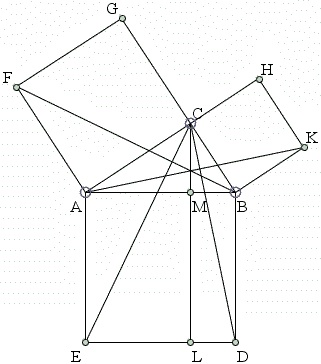
\includegraphics[scale=.55]{graphics/euclid.jpg}
%     \caption{Euclid's proof of the Pythagorean Theorem}
%     \label{fig:1.5}
% \end{figure}

This element of Kant's thought, however, is not without precedent in Aristotle. In Book \textsc{iii} of \emph{De Anima}, Aristotle claims that just as perception is the assimilation of sensible form, the passive intellect is the assimilation of intelligible form. Moreover, just as the assimilation of sensible form requires a medium, so too does the assimilation of intelligible form. Specifically, Aristotle claims that it is the activity of the active intellect that functions as the medium through which intelligible forms may be assimilated. So the acquisition of knowledge, as Aristotle conceives of it, involves the activity of the understanding---a mode of spontaneity that makes possible the reception of intelligible form.

According to Aristotle, the difference in object between perception and know\-ledge explains why perception and knowledge are the exercise of different kinds of capacities. Since the objects of perception are external particulars, our perceptual capacities are only ever exercised in the presence of such particulars. In this way, perception is a mode of sensitivity to particulars in the natural environment that not only exist independently of being perceived but whose natures and powers obtain independently of being perceived as well. But since the objects of knowledge, and cognition more generally, are universal, the exercise of our epistemic and cognitive capacities need not be constrained in this way by the particular case.

% subsection particular (end)

\subsection{Remote} % (fold)
\label{sub:remote}

There are two senses in which the objects of perception may be remote:
\begin{enumerate}[(1)]
	\item The object of perception may be remote from the perceiver
	\item The object of perception may be remote from the organ of sensation
\end{enumerate}
These claims are logically distinct. Only the latter is a direct challenge to the Empedoclean principle, to be perceptible is to be palpable to sense. Suppose as Aristotle claims, that the object of perception must be remote from the organ of sensation. The object of perception may yet be in contact with the perceiver.

In some passages, the remoteness of perceptual objects is understood one way, but not in all passages. When Aristotle criticizes the Empedoclean principle, he has in mind the remoteness of the object of perception from the organ of sensation. When Aristotle distinguishes touch and taste as operating by contact in contrast with the distal senses such as sight and audition which operate not through direct contact but through an intervening medium, he has in mind the remoteness of the object of perception from the perceiver. Indeed there are correlative notions of a medium. When the remoteness at stake is the remoteness of the object of perception from the sense organ, this will notoriously lead Aristotle to maintain that the perceiver's flesh is a medium through which the tangible qualities of bodies are felt. But when the remoteness at stake is the remoteness from the perceiver, this will lead to Aristotle distinguishing touch and taste from sight and audition as not requiring a medium for their operation. 

There is no inconsistency here. Touch and taste are distinguished from sight and audition in that only the latter require the existence of an external medium for their operation. But this is consistent with touch and taste requiring, at the same time, an internal medium for their operation. Indeed, it is Aristotle's opposition to the Empedoclean principle that makes it possible for him to use contact to distinguish kinds of sensory modalities. If all sensation operates by contact with its object, as Empedocles maintains, then it would be impossible to distinguish the contact senses and the distal senses in the way that Aristotle recommends. The Aristotelean distinction between the contact senses and the distal senses presupposes and relies upon Aristotle's cases against the Empedoclean principle, to be perceptible is to be palpable to sense.

The distinction between the contact and distal senses having been made, Aristotle will argue that the distal senses are essential for animals with the capacity for locomotion:
\begin{quote}
	Both these senses [the contact senses, touch and taste], then, are indispensable to the animal, and it is clear that without touch it is impossible for an animal to be. All the other senses subserve well-being and for that very reason belong not to any and every kind of animal, but only to some, e.g. those capable of forward movement must have them; for, if they are to survive, they must perceive not only by immediate contact but also at a distance from the object. (Aristotle, \emph{De Anima} \textsc{iii} 12 434\( ^{b} \)22--25; Smith in \citealt[62]{Barnes:1984uq})
\end{quote}
In animals capable of locomotion, since nature distributes capacities in a purposive manner (\emph{De Anima} \textsc{iii} 12 434\( ^{a} \)81--82), there is also the capacity to perceive at a distance so that the animal may move towards vital sources of nourishment, say. If animals capable of locomotion lacked the capacity to perceive at a distance they would not survive since they lack, as well, the capacity to draw nourishment from where they are rooted like plants and stationary animals. They must move towards their nourishment and flee from their predators. The capacity to perceive at a distance is necessary for our well-being and continued existence.

% subsection remote (end)

% section sensible_qualities_of_remote_external_particulars (end)

\section{Against the Empedoclean Principle} % (fold)
\label{sec:against_the_empedoclean_principle}

In its original form, Empedoclean puzzlement about the sensory presentation of remote objects is generated by a general conception of sensory awareness---the ingestion model. Specifically, given the ingestion model, a question arises about how to coherently combine the distal character of the objects of sight with a key feature of that model, the principle that to be perceptible is to be palpable to sense. A cogent argument against that principle would undermine whatever puzzlement that it generates. 

Aristotle believes that a simple empirical observation constitutes such an argument:
\begin{quote}
	If what has colour is placed in immediate contact with the eye, it cannot be seen. (Aristotle, \emph{De Anima} \textsc{ii} 7 419\( ^{a} \)13--14; Smith in \citealt[]{Barnes:1984uq})
\end{quote}
If a colored particular's being in contact with the eye blinds the perceiver to its color, then the colored particular must be at a distance from the perceiver if its color is to be seen. And if the colored particular is remote from the perceiver, an intervening medium is necessary in order for the the organ of sight to be acted upon, as it must be if it is to be a mode of sensitivity:
\begin{quote}
	Colour sets in movement what is transparent, \emph{e.g.} the air, and that, extending continuously from the object of the organ, sets the latter in movement. Democritus misrepresents the facts when he expresses the opinion that if the interspace were empty one could distinctly see an ant on the vault of the sky; that is an impossibility. Seeing is due to an affection or change of what has the perceptive faculty, and it cannot be affected by the seen colour itself; it remains that it must be affected by what comes between. Hence it is indispensable that there be something in between---if there were nothing, so far from seeing with greater distinctness, we should see nothing at all. (Aristotle, \emph{De Anima} \textsc{ii} 7 418\( ^{b} \)13--22; Smith in \citealt[33--34]{Barnes:1984uq})
\end{quote}

While Empedocles is not mentioned in this passage, Democritus instead being singled out for criticism, when this issue is raised again in \emph{De Sensu}, the connection with Empedocles is made explicit:
\begin{quote}
	To say with the ancients that colours are emanations, and that the visibility of object is due to such a cause, is absurd. For they must, in any case, explain sense-perception through touch; so that it were better to say at once that visual perception is due to a process set up by the perceived object in the medium between this object and the sensory organ; due, that is, to contact, not to emanations. (Aristotle, \emph{De Sensu} \textsc{iii} 440\( ^{a} \)16--21; Beare in \citealt[9]{Barnes:1984uq})
\end{quote}

Aristotle is making negative and positive claims in these passages. The negative claim is that an object's contact with the eye is incompatible with its being seen. The positive claim is that the eye is acted upon not by the object seen but by the intervening medium. By Aristotle's lights, Democritus and Empedocles make distinct, if related mistakes. Each fail to appreciate the necessity of a medium acting upon the organ of sight, but they do so for different reasons. Whereas Democritus is committed to the denial of the positive claim, Empedocles is committed to the denial of the negative claim.

First, consider the positive claim that the existence of a suitable medium is necessary for sight. This is meant to follow from the conjunction of the negative claim and a thesis about the nature of perceptual capacities. Specifically, perceptual capacities are a mode of sensitivity. They are reactive capacities. As such, they are only ever exercised when acted upon by something external. Since contact with a colored particular precludes perception of the particular and its color, the eye cannot be acted upon by the colored particular. But the eye must be acted upon if the colored particular is to be seen. Only the intervening medium could act upon the organ of sight in the requisite manner. In the absence of an intervening medium, nothing would act upon the eye, and nothing would be seen.

Democritus is thus insensitive to the way in which sight is a reactive capacity. Since sight is a reactive capacity, the organ of sight must be acted upon if the subject's potential for sight is to be actualized. But the void that Democritus postulates precludes there being anything that could act upon the eye, the organ of sight. Democritus is thus committed to denying the positive claim that in seeing a colored particular the intervening medium acts upon the organ of sight.

Second, consider Aristotle's negative claim that a particular's contact with the eye is incompatible with seeing its color.  We can distinguish specific and more general versions of the negative claim. Whereas the specific claim is about color, the more general claim is about the objects of sense more generally, and thus holds of sound and smell as well:
\begin{enumerate}[(1)]
	\item A colored particular is imperceptible if it is in contact with the organ of sight;
	\item A sensible particular is imperceptible if it is in contact with the relevant sense organ.
\end{enumerate}

Consider first the specific claim about color. Here the thought is that in order to have a colored particular in view the perceiver must have a view on that colored particular. A colored particular's contact with the eye, the organ of sight, would preclude a point of view on that particular and its color. It is a necessary condition for a perceiver to have a point of view on a particular and its color that the particular be at a distance from the perceiver. To have a point of view on something is for that thing to be remote from one. 

The specific claim about color is echoed in Aristotle's criticism of the likeness theory. According to the likeness theory, perception is to be explained in terms of the similarity of the elements with which the sense organ and the object of sense are composed. The likeness theory is subject to a range of criticisms especially in the first book of \emph{De Anima}; however, in \emph{De Sensu}, Aristotle writes:
\begin{quote}
	For certainly it is not true that the beholder sees, and the object is seen, in virtue of some merely abstract relationship between them, such as that between equals. For if it were so, there would be no need that either should occupy some particular place; since to the equalization of things their being near to, or far from, one another makes no difference. (Aristotle, \emph{De Sensu} \textsc{iii} 446\( ^{b} \)10--13; Beare in \citealt[20]{Barnes:1984uq})
\end{quote} 
Aristotle's complaint, here, is that equality, understood as complete compositional similarity of the sense organ and the object of sense, does not afford the perceiver with a point of view. The perceiver's point of view on a particular depends upon that particular being at some distance from the perceiver. Moreover, that point of view varies as the object of sense is near or far. However, compositional similarity does not determine that the object of sense is any particular distance from the perceiver and hence fails to determine a point of view on that particular.

At least with respect to color vision, then, Aristotle's rejection of the Empedoclean principle, to be perceptible is to be palpable to sense, is unequivocal. Far from being a necessary condition on sight, contact with a colored particular blinds us to that particular and its color. Consistent with that denial, the Empedoclean principle may nevertheless be true of other objects of sense, such as taste and touch. A more thoroughgoing rejection of the principle, then, would regard the specific claim about color as an instance of the more general claim about the objects of sense. An object being in contact with the relevant sense organ, far from being a necessary condition for sensing that object, precludes it from being the object of sensation. The claim here is general, applicable to all objects of sense---contact precludes sensation, to be palpable is to be imperceptible.

While Aristotle at least makes the specific claim about color, his complete case against the Empedoclean principle, to be perceptible is to be palpable to sense, may involve the more general claim. The distinction between the specific and more general claim is relevant not only to the depth of Aristotle's case against the Empedoclean principle, but the distinction is relevant as well as to the relative plausibility of these claims. Even if the more general claim should prove to be false---of taste or touch, say---the specific claim about color may yet be true. It could turn out that vision is distinctive in being a sensory mode of presentation of the qualities of remote objects. Thus, for example, \citet[]{Broad:1952kx} claims that a comparative phenomenology of our sensory capacities supports this view (even if he thinks that our phenomenology is misleading in this regard, and that the distinctive phenomenological character of vision is ultimately undermined by the common causal mechanisms underlying all of our sensory capacities). Indeed, Broad might fairly point out that the rationale so far offered for the specific denial about color appeals to a feature specific to vision, that in order to see something, the subject must have a point of view on it.

Aristotle's discussion of the special senses makes plain that he endorses the more general claim that contact precludes perception, that to be palpable is to be imperceptible:
\begin{quote}
	The same account holds also of sound and smell; if the object of either of these senses is in immediate contact with the organ no sensation is produced. In both cases the object sets in movement only what lies between, and this in turn sets the organ in movement: if what sounds or smells is brought into immediate contact with the organ, no sensation will be produced. The same, in spite of all appearances, applies also to touch and taste \ldots\ (Aristotle, \emph{De Anima} \textsc{ii} 7 419\( ^{a} \)26--34; Smith in \citealt[34]{Barnes:1984uq})
\end{quote}
And later, in a discussion of why humans can only smell when they inhale, the general denial of the Empedoclean principle is invoked as a constraint on an adequate explanation:
\begin{quote}
	\ldots\ it is common to all not to perceive what is in immediate contact with the organ of sense \ldots\ (Aristotle, \emph{De Anima} \textsc{ii} 9 421\( ^{b} \)16--18; Smith in \citealt[38]{Barnes:1984uq})
\end{quote}

Indeed, Aristotle's conviction that to be palpable is to be imperceptible drives him to deny that flesh is the organ of touch:
\begin{quote}
    In general, flesh and the tongue are related to the organs of touch and taste, as air and water are to those of sight, hearing, and smell. Hence in neither the one case nor the other can there be any perception of an object if it is placed immediately upon the organ, e.g. if a white object is placed on the surface of the eye. This again shows that what has the power of perceiving the tangible is seated inside. (Aristotle, \emph{De Anima \textsc{ii} 11 423\( ^{b} \)}18--23; Smith in \citealt[42]{Barnes:1984uq})
\end{quote}
This is a surprising claim. One may be forgiven for thinking that Aristotle has taken his opposition to the Empedoclean principle too far. But let us see what can be said on behalf of it.

First, consider the following examples of Dennett's:
\begin{quote}
    Blindfold yourself and take a stick (or a pen or pencil) in your hand. Touch various things around you with this wand, and notice that you can tell their textures effortlessly---as if your nervous system had sensor out at the tip of the wand. \ldots\ For an even more indirect case, think of how you can feel the slipperiness of an oil spot on the highway under the wheels of your car as you turn a corner. The phenomenological focal point of contact is the point where the rubber meets the road, not any point on your innervated body, seated, clothed, on the car seat, or on your gloved hands on the steering wheel. \citep[47]{Dennett:1993ce}
\end{quote}
These are nice examples of artificially extending tactile consciousness beyond the limits of the perceiver's innervated body. We feel the texture at the end of the pen, but not by feeling the pen in our hand. If we accept Dennett's description of these cases, then contact with flesh is not necessary for something to be the object of tactile awareness. While a good objection to the conjunction of Empedoclean principle and the claim that flesh is the organ of touch, this is too weak to establish Aristotle's counterprinciple, to be palpable is to be imperceptible. Contact with the organ of touch may not be necessary for something to be the object of tactile awareness, but that is consistent with contact being sufficient for tactile awareness. Nevertheless, Dennett's examples remove an important obstacle to the acceptance of Aristotle's position. They make vivid the possibility of tactile awareness through a medium of objects remote from the organ of touch.

Aristotle's bold thought is that we are always already in the position described by Dennett. When we feel the texture of a body with our fingertips, the phenomenological point of contact is remote from the organ of touch, no less than when we feel the texture of that same body with a pen. Like the pen, the flesh of our fingertips is not the organ of touch but the medium through which the texture of the body is felt. Aristotle's conception of touch is an internalization of the model provided by Dennett's examples. Just as the phenomenological point of contact can be extended from the sense organ by means of an external medium, the phenomenological point of contact is always already extended from the sense organ by means of an internal medium. The perceiver's flesh is an internal medium, the organ of touch residing within. Indeed, Aristotle appeals to the internalization of an external medium to motivate the claim that flesh is not the organ of touch but its medium:
\begin{quote}
    To the question whether the organ of touch lies inward or not (i.e. whether we need look any farther than the flesh), no indication can be drawn from the fact that if the object comes into contact with the flesh it is at once perceived. For even under present conditions if the experiment is made of making a sort of membrane and stretching it tight over the flesh, as soon as this web is touched the sensation is reported in the same manner as before, yet it is clear that the organ is not in this membrane. If the membrane could be grown on to the flesh, the report would travel still quicker. (Aristotle, \emph{De Anima} \textsc{ii} 11 422\( ^{b} \)34--423\( ^{a} \)6; Smith in \citealt{Barnes:1984uq})
\end{quote}

If Aristotle's counterprinciple, to be palpable is to be imperceptible, can be sustained in its fully generality, then the Empedoclean principle, to be perceptible is to be palpable to sense, not only involves an overgeneralization from a paradigm case but a misconception of it as well. According to Aristotle, the principle fails even of touch. The tangible is not palpable to touch. The apparent aporetic character of this doctrine, perhaps unsurprisingly, elicits in \citet[6]{Derrida:2005aa} the following Joycean play: ``one keeps asking oneself \ldots\ above all what an `intangible' accessible to touch is---a still touchable un-touchable. How to touch the untouchable?'' The tangible is merely palpable to the internal medium, the perceiver's flesh, the organ of touch residing within, at or near the heart. That the Empedoclean principle not only involves an overgeneralization from a paradigm case but a misconception of it as well is philosophically significant. Specifically, it bears on the significance of the tactile metaphors with which we unselfconsciously characterize sensory presentation. Grasping may be a paradigm case of sensory presentation. This is why the Giants are literally grasping rocks and trees as they are strenuously affirming their case. And Aristotle agrees that felt resistance to touch is primitively compelling. Without touch it is not possible for an animal to exist, whereas the distal senses are for the animal's well-being (\emph{De Anima} \textsc{iii} 13 433\( ^{b} \)31--434\( ^{a} \)10). According to Aristotle, touch is primitively compelling because of its existential character. Grasping may be a paradigm case of sensory presentation, but not because it involves an object being in contact with the sense organ, as the ingestion model would have it, but because objects grasped are presented to us in a primitively compelling manner. Phenomenologically vivid and primitively compelling instances of grasping are paradigms of sensory presentation not because the object grasped is palpable to the organ of touch, but because it is precisely the presentation of the object grasped. However, as we shall see in the next section, this just raises the generalized form of Empedoclean puzzlement: What could sensory presentation be if it is not just being palpable to sense?

Can Aristotle's counterprinciple, to be palpable is to be imperceptible, be sustained in its full generality? Aristotle's empirical argument consisted in the observation that a colored particular is not seen when placed upon the eye. He varies this argument with some of the other sensory modalities. He thus offers variants of this argument for audition and smell. A sounding object placed upon the ear is not heard, nor is a pungent object smelled when in contact with the organ of smell. However, no such argument is offered for touch. So Aristotle's empirical argument, even if conceded to be a good argument for the specific claims about color, sound, and smell, is insufficient to establish the more general claim. This weakness of his argument has been well observed by previous commentators. What is less well appreciated, I think, is the dialectical constraints that Aristotle is operating within. Specifically, he simply could not offer a tactile variant of the empirical argument. After all, whether in grasping the object grasped is in contact with the sense organ is precisely what is at issue between Aristotle and his opponents. But any tactile variant of the empirical  argument must at least implicitly rule on this matter in the very description of the case. So Aristotle is debarred from offering the tactile variant of the empirical argument. Within these constraints, Aristotle has offered variants of the empirical argument for non-tactile sensory modalities with the hope that they display sufficient regularity to be projected onto the tactile case. Even so understood, Aristotle's case for his counterprinciple, to be palpable is to be imperceptible, is subject to criticism. In smelling an odor, particulate matter is in contact with the nasal membrane, and audible vibrations may be transmitted via contact with the tympanic membrane. Moreover, the claim about color received what support it did from a feature specific to vision---that in order to see something, the perceiver must have a view on it. In the end, it must be conceded that Aristotle has a better case for the more specific claim about color than for the more general claim.

There may, however, be a further aspect of Aristotle's case. Aristotle's belaboring and not always completely resolving the puzzling and aporetic character of touch can be read as an attempt to undermine the Empedoclean principle (compare \citealt[``When our eyes touch \ldots'']{Derrida:2005aa}). If to be perceptible is to be palpable to sense, then all sensation is a kind of touch. Conceiving of non-tactile modes of sensory awareness on the model of touch will seem explanatory insofar as touch is antecedently understood to be an unproblematic mode of perception. Thus \citet[39]{Lindberg:1977aa} observes that in the ancient world ‘‘the analogy of perception by contact in the sense of touch seemed to establish to nearly everybody’s satisfaction that contact was tantamount to sensation, and it was not apparent that further explanation was required.’’ The \emph{aporiai} concerning touch undermine that assumption. And if further explanation is required, then we can no longer simply assume that contact is tantamount to sensation.

Even if Aristotle's cases against the Empedoclean principle does not have the depth that it aspires to, even if Aristotle has not established his counterprinciple, to be palpable is to be imperceptible, as long as the specific claim about color is true, as long as contact with a colored particular precludes perception of the particular and its color, then the falsity of the Empedoclean principle, to be perceptible is to be palpable to sense, is established. What is more, Empedoclean puzzlement, in its original form, arose specifically about color vision. Sight seems to present the perceiver with the colors of remote external particulars, but how could this be if what it is for something to be perceptible is for it to be palpable to sense? Showing that the Empedoclean principle fails of color perception is philosophically significant, since Empedoclean puzzlement, in its original form, arises from color perception presenting itself as a mode of awareness of the colors of remote external particulars. 

Even if Aristotle has not established his counterprinciple, to be palpable is to be imperceptible, if his empirical argument involving colored particulars succeeds, if he has established that a colored particular's contact with the eye blinds the perceiver to the particular and its color, then the Empedoclean principle, to be perceptible is to be palpable to sense, is false. But if sensory presentation is not contact with the perceptive part of the soul located within, then what is it? An why does it remain apt to think of color perception as mode of assimilation, as visually taking in the colors arrayed in the scene before one? While Empedoclean puzzlement, in its original form, may have been dispensed with, the questions that subsequently arise are grounds for residual puzzlement.

% section against_the_empedoclean_principle (end)

\section{The Generalized Form of Empedoclean Puzzlement} % (fold)
\label{sec:the_generalized_form_of_empedoclean_puzzlement}

In its original form, Empedoclean puzzlement about the sensory presentation of remote objects consists in the apparent tension between two claims:
\begin{enumerate}[(1)]
    \item The objects of color perception are qualities of external particulars located at a distance from the perceiver.
    \item \emph{The Empedoclean principle}: To be perceptible is to be palpable to sense---in order for something to be the object of perception it must be in contact with the relevant sense organ.
\end{enumerate}
Aristotle response to the initial form of Empedoclean puzzlement is to reject the Empedoclean principle, to be perceptible is to be palpable to sense. In its stead he proposes the Aristotelian counterprinciple---to be palpable is to be imperceptible. 

Even having rejected the ingestion model, it remains natural to think of seeing as taking in the external scene before one. Thus, Aristotle retains a conception of perception as a mode of assimilation even as he rejects the ingestion model. This gives rise to a residual puzzlement. How can one take in what remains external? And if one can, what could taking in mean, here, such that one could? Empedoclean puzzlement, in its most general form, consists in the persistence of this latter question. How does Aristotle's account address this generalized form of Empedoclean puzzlement? Reflection on the specific way in which the residual puzzlement arises for Aristotle provides some evidence.

Aristotle in rejecting the ingestion model denies that perception is the mode of assimilation of anything material. But there are distinguishable senses of material in play both in the ingestion model and Aristotle's argument against the Empedoclean principle. First, material might mean physical or physical matter more narrowly (fields are physical but not matter). Second, material might mean matter in Aristotle's technical sense associated with his hylomorphic theory. Chromatic effluences assimilated by the organ of sight are material in both senses. Chromatic effluences are physical matter, they at least have elemental composition. And chromatic effluences are in-formed matter, at least by Aristotle's lights. The distinctive magnitudes of chromatic effluences are the forms enmattered by them. So too with the colored object blinding the subject to its color when placed upon the eye. The colored object is both physical matter and in-formed matter. The colored object has an elemental composition. Moreover, the color of the object is a sensible form enmattered in the object.

These distinct senses of material provide distinct potential grounds for rejecting the Empedoclean principle. They thus also provide distinct potential contrasts with Aristotle's alternative conception of perception. First, consider the distinct potential grounds for rejecting the Empedoclean principle, to be perceptible is to be palpable to sense. Is what precludes perception contact with physical matter or in-formed matter? If we confine our attention to Aristotle's case, the colored object blinding the subject to its color when placed upon the eye, then Aristotle need not choose between them. Contact with physical matter and contact with in-formed matter may both be sufficient to preclude perception. But if we look forward to Aristotle's definition of perception as the assimilation of the form without the matter of the perceived object, then it is compelling to understand the contrast in terms of in-formed matter. 

This is weak indirect evidence that Aristotle's definition of perception as the assimilation of sensible form without the matter of the object of perception is meant to address the generalized form of Empedoclean puzzlement. It is meant to be the sense in which the subject takes in the scene before them. More specifically, it is meant to be the sense in which the subject takes in what remains external. The subject assimilates the sensible form of the object while leaving its matter in place. Aristotle's definition, so interpreted, as addressing the generalized form of Empedoclean puzzlement, is making an important metaphysical claim about the nature of sensory presentation.


% section the_generalized_form_of_empedoclean_puzzlement (end)


% chapter perception_at_a_distance (end)
